\begin{figure}[H]
\centering
\caption{Connectivity and Wage Changes: Raw Connectivity}
\label{fig:scatter_resid_wages_raw}

\begin{threeparttable}

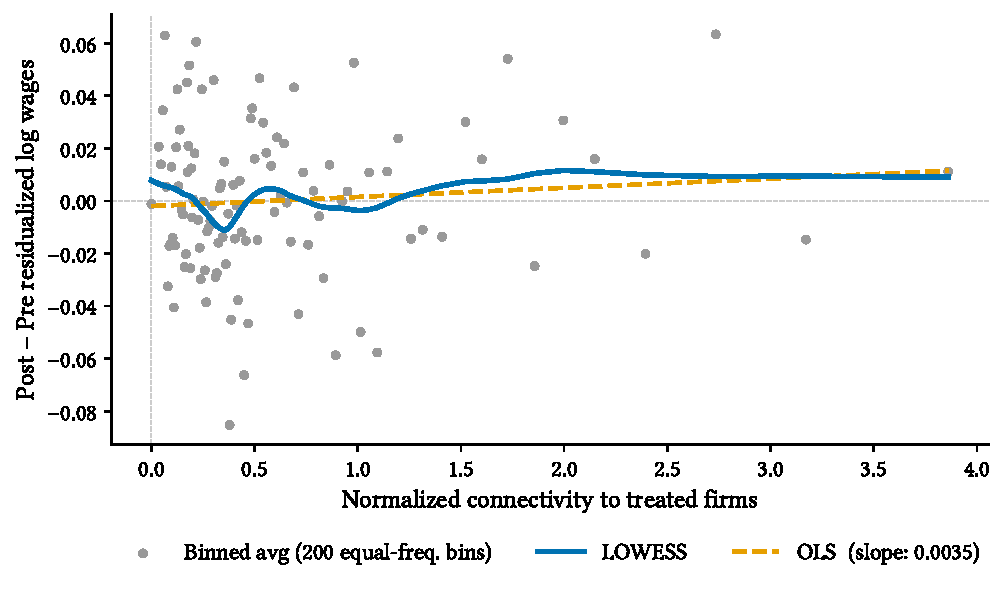
\includegraphics[width=0.75\textwidth]{scatter_resid_wages_raw.pdf}

\begin{tablenotes}
\footnotesize
\item \textit{Notes:} This figure plots the firm-level difference in residualized log December wages (post minus pre Súmula 277) against normalized connectivity to treated firms (\texttt{totaltreat\_pw\_norm}). Firms are grouped into 200 equal-frequency bins by connectivity; each dot represents the bin average of both axes. The solid blue line is a LOWESS fit (bandwidth $= 0.4$) and the dashed yellow line is an OLS reference line. The x-axis is trimmed at the 99th percentile of connectivity.
\end{tablenotes}

\end{threeparttable}
\end{figure}
